\documentclass[uplatex,dvipdfmx,titlepage]{jsarticle}
\usepackage[dvipdfmx]{graphicx}
\usepackage{amsmath,amssymb}
\usepackage{bm}
\usepackage{enumitem} 
% lable絶対かえたほうがいい
\title{固体力学の実験}
\author{京都大学工学部物理工学科 1025363386 伊藤温大}
\date{\today}

\begin{document}
\maketitle

\tableofcontents
\clearpage


\section{はじめに}
本レポートでは、固体力学に関する光弾性法による応力場の可視化と応力集中係数の評価について、その結果および実験課題について報告する。

\section{光弾性法による応力場の可視化と応力集中係数の評価}

\subsection{目的}
曲げ応力を受ける梁の干渉縞の測定を行い、切り欠き部における応力集中係数を評価する。それによって光弾性法の原理を理解する。

\subsection{実験方法}
以下の手順で測定を行った。

\subsubsection*{課題1：基準試験片の光弾性画像と縞次数の解析}
切り欠きの無い基準試験片に対して錘の質量、支点位置、視野の明暗を調節し、光弾性画像を撮影することで縞次数を解析した。\\
実験に際して以下の器具を使用した。図\ref{fig:specimen}に示すような、ポリカーボネート製の梁を試験片として使用した。\\
図の上から切り欠きなし、切り欠きの半径$\rho=1, 2, 4, 8$ mmである。

\begin{figure}[htbp]
    \centering
    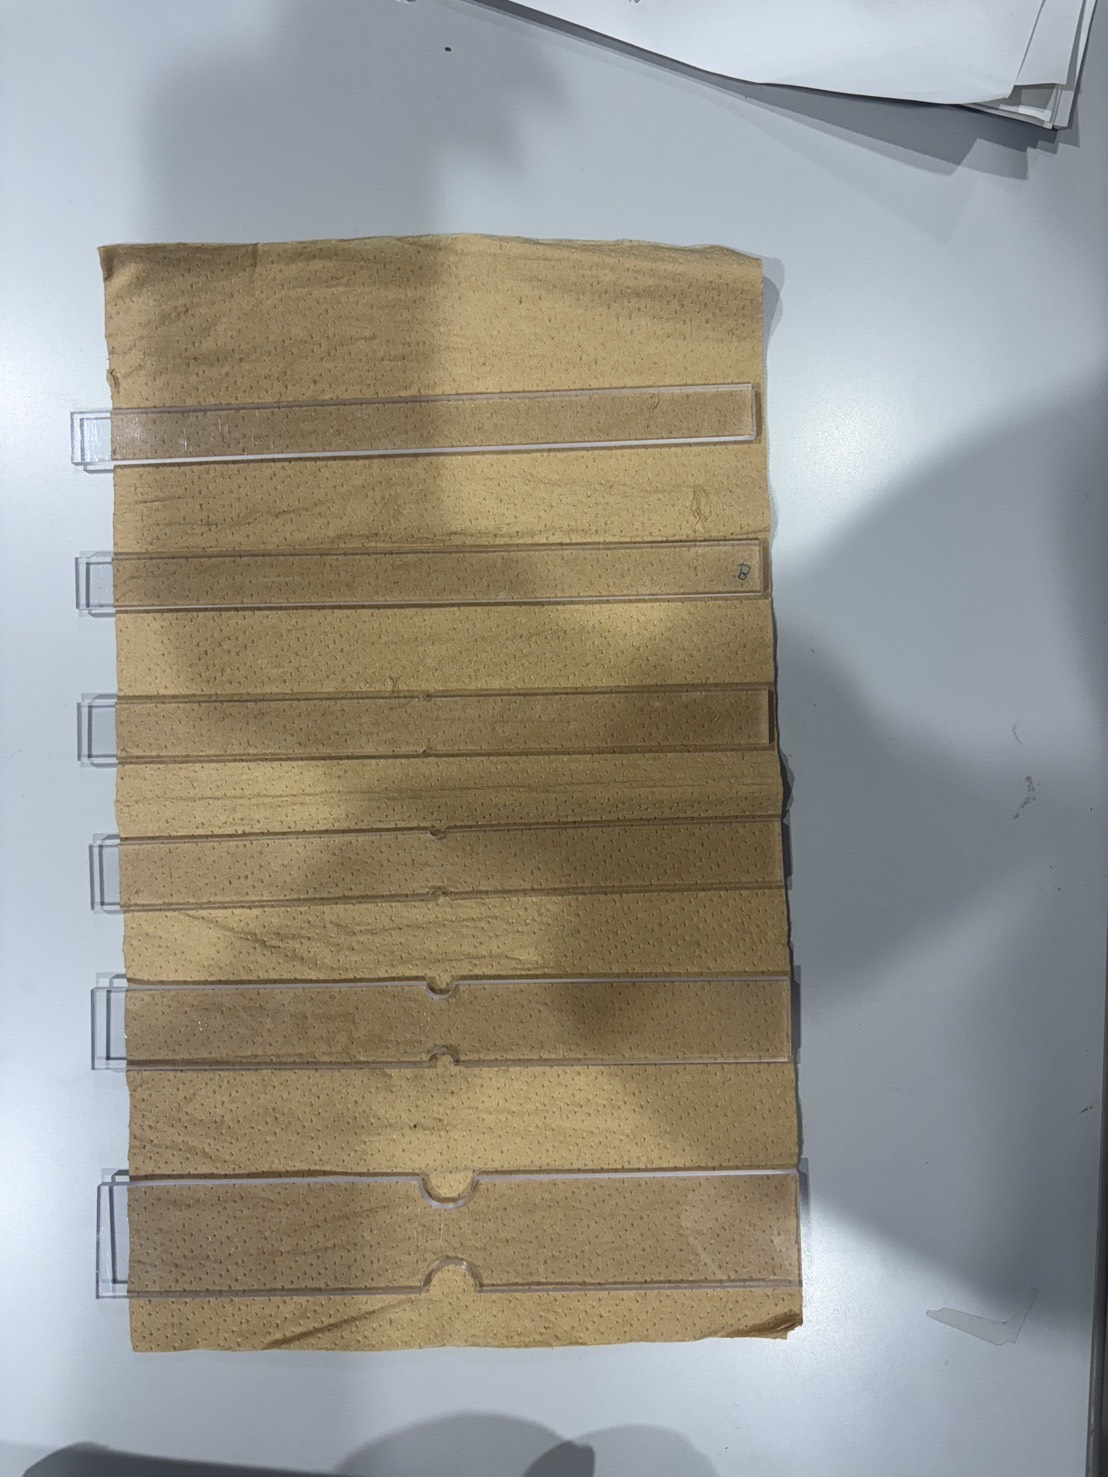
\includegraphics[width=8cm]{実験試験片.jpg}
    \caption{試験片（上から切り欠きなし、切り欠きの半径$\rho=1, 2, 4, 8$）}
    \label{fig:specimen}
\end{figure}
%錘と光学系について同じ図をめんしょんするようにする
また、図\ref{fig:bending_machine}の左にある曲げ試験装置を用いて4点曲げ試験を行った。この装置では直径10 mmのピン4本で試験片を支持し、上部から錘をのせることで荷重を作用させる。このとき錘の質量を$W$ (kg)、支点位置を$e$ (cm)として$W, e$を変化させ、実験を行った。\\
実験で使用した光学系は以下のとおりである。
\begin{enumerate}[label=\arabic*.]
    \item He-Ne レーザー
    \item レーザービームエキスパンダ
    \item 平凹レンズ
    \item 平凸レンズ
    \item CMOSカメラ
\end{enumerate}
これらの全体像は以下のようである。
\begin{figure}[htbp]
    \centering
    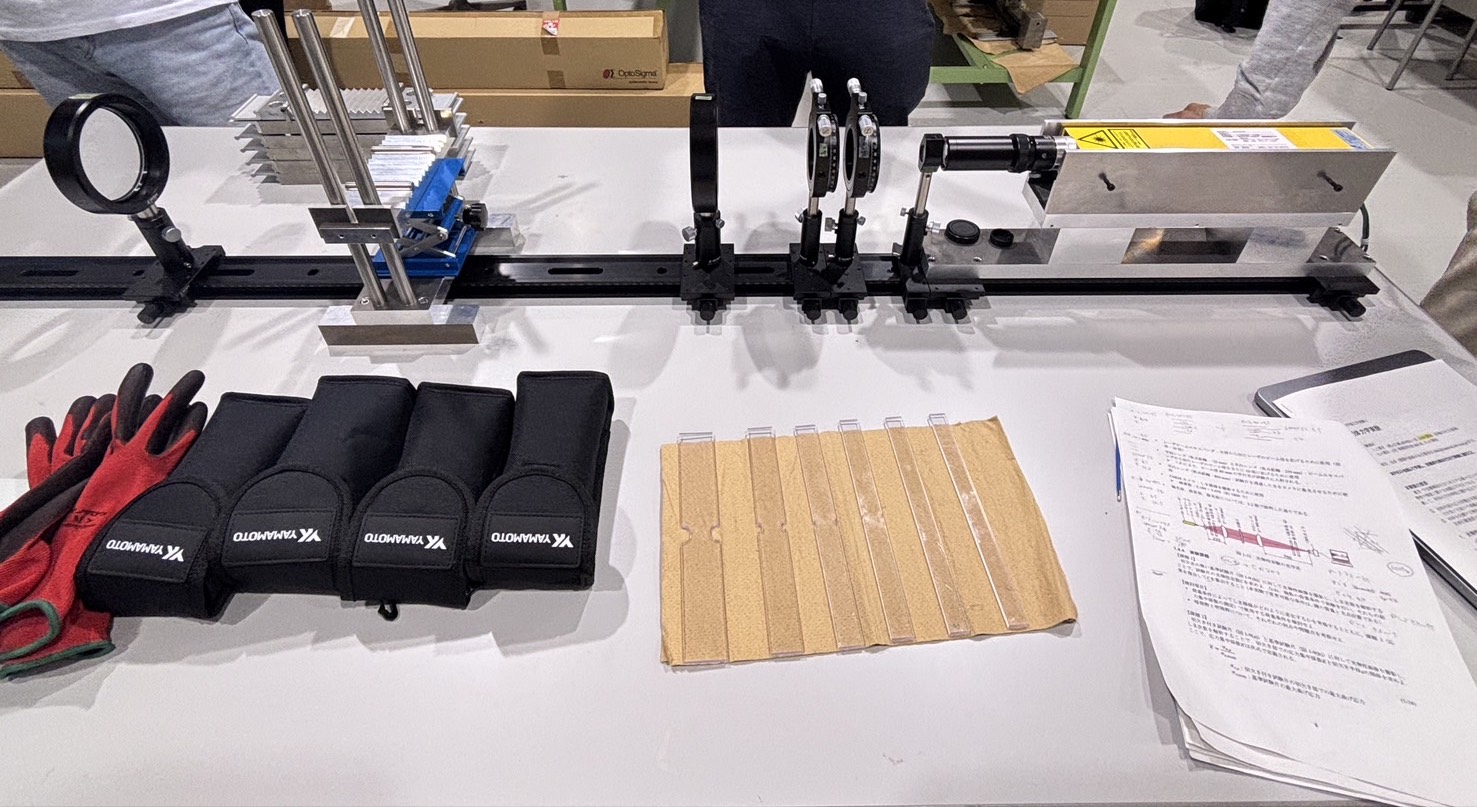
\includegraphics[width=8cm]{実験全体写真2.jpg}
    \caption{4点曲げ試験装置の概略図}
    \label{fig:bending_machine}
\end{figure}
%いったんこの設定条件と結果をひとまとめにする
% TO DO-これを分割するか考える
切り欠きの無い基準試験片に対して加えた錘の質量、支点位置、視野の明暗の設定条件、
これらより、縞次数と位置の関係をまとめると以下の図のようになった。\ref{tab:conditions}のようになった。
\begin{table}[htbp]
    \centering
    \caption{実験条件および測定結果}
    \label{tab:conditions}
    % \resizebox{\textwidth}{!} で表をページ幅に自動調整します
    \resizebox{\textwidth}{!}{
    \begin{tabular}{ccccccccccccccc}
    \hline
    No. & 視野 & $\lambda$ [m] & $h$ [m] & $e$ [cm] & $W$ [kg] & $y_1$ & $y_2$ & $y_3$ & 縞次数1 & 縞次数2 & 応力1 & 応力2 & $\alpha_1$ & $\alpha_2$ \\ \hline
    1 & 明 & 6.33E-07 & 0.015 & 4.5 & 2 & 4.3 & 6.8  & 6.2 & 1.19 & 1.60 & 6.42E-11 & 8.59E-11 & 64.22 & 85.92  \\
    2 & 明 & 6.33E-07 & 0.015 & 4.5 & 3 & 5.5 & 7.4  & 4.2 & 1.81 & 2.26 & 6.49E-11 & 8.11E-11 & 64.91 & 81.14  \\
    3 & 明 & 6.33E-07 & 0.015 & 4.5 & 5 & 6.7 & 10.3 & 2.5 & 3.18 & 4.62 & 6.84E-11 & 9.94E-11 & 68.45 & 99.44  \\
    4 & 明 & 6.33E-07 & 0.015 & 6.5 & 3 & 6.5 & 10.5 & 2.8 & 2.82 & 4.25 & 7.01E-11 & 1.06E-10 & 70.07 & 105.55 \\
    5 & 暗 & 6.33E-07 & 0.015 & 6.5 & 3 & 7.6 & 9    & 2.8 & 2.71 & 3.21 & 6.74E-11 & 7.98E-11 & 67.41 & 79.83  \\ \hline
    \end{tabular}
    }
\end{table}
%TO DO:以下のコードを成形し、課題1の理論の導出に沿った形にする
図1-8に示されるような対称四点曲げを受ける梁において、内側の支点間（$e < x < L-e$）では純粋曲げの状態となり、曲げモーメント $M$ とせん断力 $F$ は以下のようになる。
\begin{align}
    M &= \frac{W}{2}e \label{eq:moment} \\
    F &= 0 \label{eq:shear_force}
\end{align}
せん断力 $F$ がゼロであるため、この区間におけるせん断応力 $\tau_{xy}$ もゼロとなる。
\begin{equation}
    \tau_{xy} = 0 \label{eq:shear_stress}
\end{equation}
したがって、垂直応力 $\sigma_x, \sigma_y$ がそのまま主応力 $\sigma_1, \sigma_2$ に対応する。また、応力の平衡方程式
\begin{equation}
    \frac{\partial \tau_{xy}}{\partial x} + \frac{\partial \sigma_y}{\partial y} = 0
\end{equation}
と梁上下平面での境界条件（$y = \pm h/2$ で $\sigma_y = 0$）を用いると、同区間での $\sigma_y$ はゼロとなる。
\begin{equation}
    \sigma_y = 0 \label{eq:sigma_y}
\end{equation}
材料力学の梁の理論より、曲げ応力 $\sigma_x$ は断面二次モーメント $I = \frac{dh^3}{12}$ を用いて $\sigma_x = \frac{M}{I}y$ と表される。式(\ref{eq:moment})と式(\ref{eq:sigma_y})を考慮すると、この区間での主応力差の絶対値は、梁の厚さ $d$ と高さ $h$ を用いて次のように表される。
\begin{equation}
    |\sigma_1 - \sigma_2| = |\sigma_x - \sigma_y| = \left| \frac{6We}{dh^3}y \right| \label{eq:stress_diff}
\end{equation}
一方、光弾性法に基づく応力－光学の法則によれば、測定されるしま次数 $N$ は主応力差と以下の関係にある。
\begin{equation}
    N = \frac{Cd}{\lambda} |\sigma_1 - \sigma_2| \label{eq:photoelastic_law}
\end{equation}
ここで、$C$ は材料の光弾性定数、$\lambda$ は光源の波長である。式(\ref{eq:stress_diff})を式(\ref{eq:photoelastic_law})に代入すると、しま次数 $N$ と中立軸からの距離 $y$ の関係式が得られる。
\begin{equation}
    N = \frac{6CWe}{\lambda h^3} |y| \label{eq:N_y_relation}
\end{equation}
式(\ref{eq:N_y_relation})は、純粋曲げ領域においてしま次数 $N$ が中立軸からの距離 $y$ に比例することを


% TO DO:全体のバランスを考える
今回の課題1については4つを明視野で、1つを暗視野で観測した。

\section{総括}
本実験を通して、光弾性法を用いた応力場の評価手法、および超音波計測による弾性係数の評価手法について...
% TODO: レポート全体のまとめを記述する


% --------------------------------------------------
% 参考文献
% --------------------------------------------------
\section*{参考文献}
\begin{enumerate}[label={[\arabic*]}]
    \item 著者名, 『書籍名』, 出版社, 発行年.
    \item 物理工学科 実験指導書, 2026.
\end{enumerate}

\end{document}